\documentclass[border=8pt]{standalone}

\usepackage{amsmath}
\usepackage{caption}
\usepackage{graphicx}

\captionsetup{
  font=small,
  labelfont=bf,
  justification=justified,
  singlelinecheck=false
}

\begin{document}
\begin{minipage}{16.6cm}
  \centering

  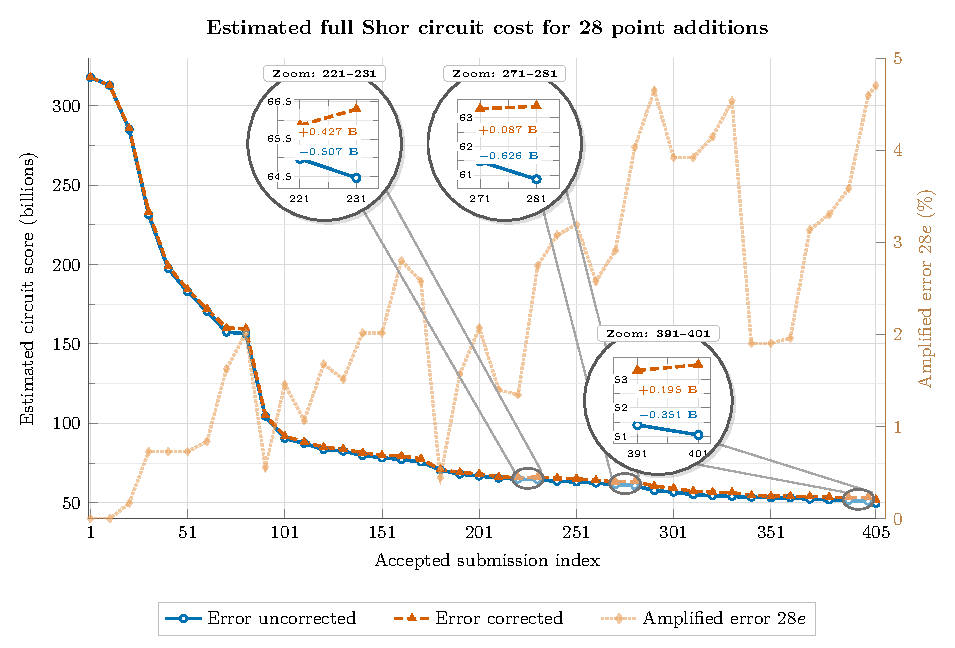
\includegraphics[width=0.97\linewidth]{../../output/pdf/shor-circuit-estimate-plot.pdf}

  \vspace{-0.15cm}
  \begin{minipage}{0.94\linewidth}
    \small
    \textbf{(a) Estimated full Shor circuit cost.}
    The raw estimate is $28Q'T'$, while the correctness-adjusted estimate is
    $28Q'T'/(1-28e)$. The faded right-axis curve shows the amplified error
    $28e$, and the circular insets expose the three local score reversals.
  \end{minipage}

  \vspace{0.35cm}

  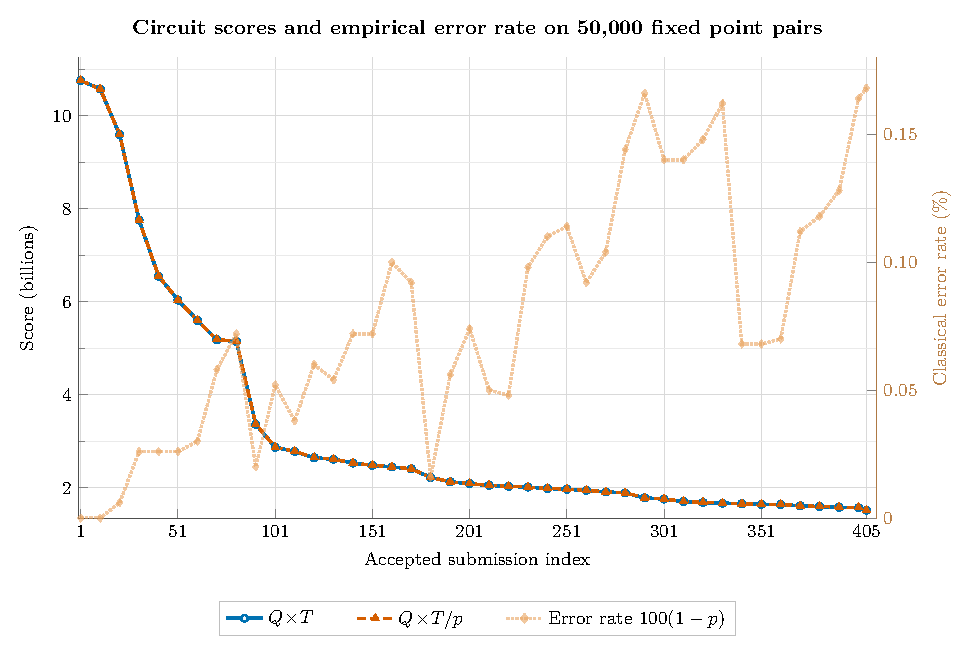
\includegraphics[width=0.97\linewidth]{../../output/pdf/qxt-error-dual-axis-plot.pdf}

  \vspace{-0.15cm}
  \begin{minipage}{0.94\linewidth}
    \small
    \textbf{(b) Point-addition circuit score.}
    The left axis compares the standard $Q\!\times\!T$ score with the
    correctness-adjusted $Q\!\times\!T/p$ score. The faded right-axis curve
    reports the measured classical error rate $100(1-p)$.
  \end{minipage}

  \vspace{0.30cm}

  \captionof{figure}{%
    Resource-cost evolution across the sampled accepted submissions. Both
    panels use the same fixed corpus of 50,000 elliptic-curve point pairs per
    commit. For the full-circuit estimate, $Q'=Q+16$, $T'=T+3\cdot2^{16}$,
    and $e=1-p$. Lower scores are better; the right axes report error-related
    quantities rather than resource costs.
  }
  \label{fig:qxt-shor-comparison}
\end{minipage}
\end{document}
